% !TEX root = ../CourseOT.tex

%%%%%%%%%%%%%%%%%%%%%%%%%%%%%%%%%%%%%%%%%%%%%%%%%%%%%%%%%%%%%%%%%%%%%%%%%%%
%%%%%%%%%%%%%%%%%%%%%%%%%%%%%%%%%%%%%%%%%%%%%%%%%%%%%%%%%%%%%%%%%%%%%%%%%%%
%%%%%%%%%%%%%%%%%%%%%%%%%%%%%%%%%%%%%%%%%%%%%%%%%%%%%%%%%%%%%%%%%%%%%%%%%%%
\section{Optimal Matching between Point Clouds}

%%%%%%%%%%%%%%%%%%%%%%%%%%%%%%%%%%%%%%%%%%%%%%%%%%%%%%%%%%%%%%%%%%%%%%%%%%%
\subsection{Monge Problem between Discrete points}
\label{sec-monge-pbm}

%%%%%%%
\paragraph{Matching problem}

Given a cost matrix $(\C_{i,j})_{i \in \range{n}, j \in \range{m}}$, assuming $n=m$, the optimal assignment problem seeks for a bijection $\si$ in the set $\Perm(n)$ of permutations of $n$ elements solving
\eql{\label{eq-optimal-assignment}
	\umin{\si \in \Perm(n)} \frac{1}{n}\sum_{i=1}^n \C_{i,\si(i)}.
}
One could naively evaluate the cost function above using all permutations in the set $\Perm(n)$. However, that set has size $n!$, which is gigantic even for small $n$. 
% Consider for instance that such a set has more than $10^{100}$ elements~\cite{Dantzig1983} when $n$ is as small as 70. That problem can therefore only be solved if there exist efficient algorithms to optimize that cost function over the set of permutations, which will be the subject of~\S\ref{s-matching}.
In general the optimal $\si$ is non-unique. 

% \begin{rem}[Uniqueness] Note that the optimal assignment problem may have several optimal solutions. Suppose for instance that $n=m=2$ and that the matrix $\C$ is the pairwise distance matrix between the 4 corners of a 2-dimensional square of side length $1$, as represented in the left plot in Figure~\ref{fig-non-unique-matching}. In that case only two assignments exist, and they share the same cost. \end{rem}

%\begin{figure}
%\centering
%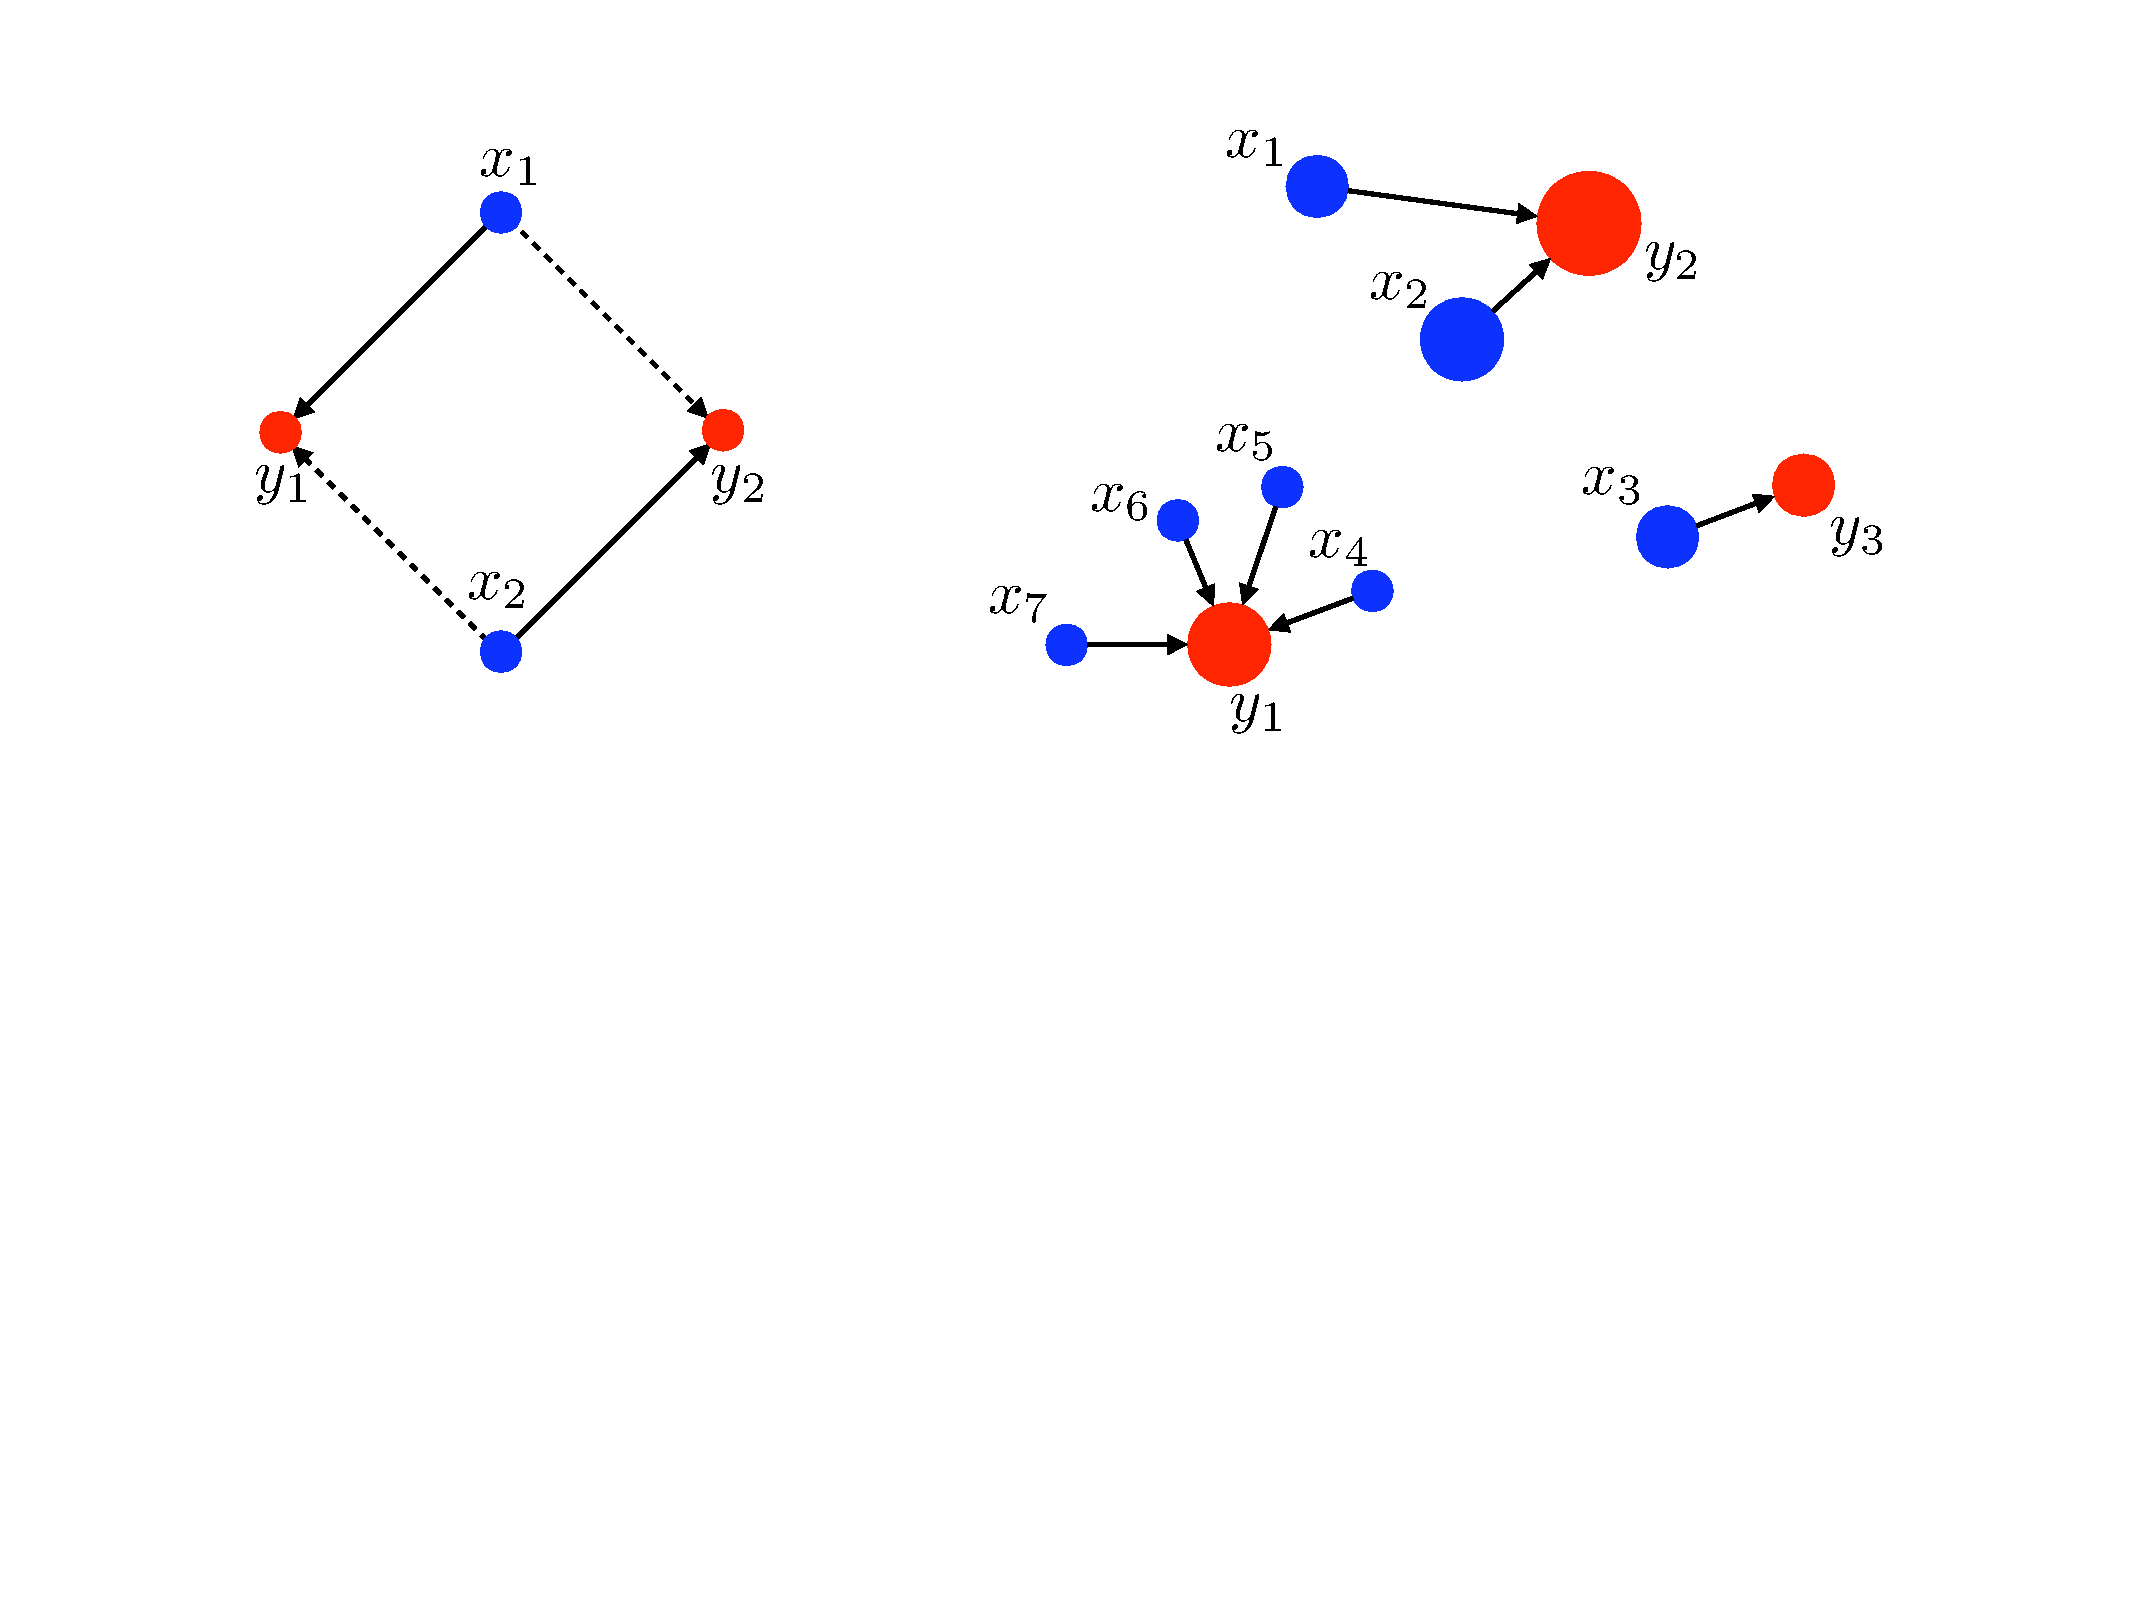
\includegraphics[width=.5\linewidth]{non-unique-optimal-matching/non-unique-optimal-matching}
%\caption{\label{fig-non-unique-matching}
%(left) blue dots from measure $\alpha$ and red dots from measure $\beta$ are pairwise equidistant. Hence, either matching $\sigma=(1,2)$ (full line) or $\sigma=(2,1)$ (dotted line) is optimal. (right) a Monge map can associate the blue measure $\alpha$ to the red measure $\beta$. The weights $\alpha_i$ are displayed proportionally to the area of the disk marked at each location. The mapping here is such that $T(x_1)=T(x_2)=y_2$, $T(x_3)=y_3$, whereas for $4\leq i\leq 7$ we have $T(x_i)=y_1$.
%}
%\end{figure}


\paragraph{1D case}

If the cost is of the form $\C_{i,j}=h(x_i-y_j)$, where $h: \RR \rightarrow \RR^+$ is  convex (for instance $\C_{i,j}=|x_i-y_j|^p$ for $p \geq 1$), one has that an optimal $\si$ necessarily defines an increasing map $x_i \mapsto x_{\si(i)}$, i.e. 
\eq{
	\foralls (i,j), \quad (x_i-y_j)(x_{\si(i)}-y_{\si(j)}) \geq 0.
}
Indeed, if this property is violated, i.e. there exists $(i,j)$ such that $(x_i-y_j)(x_{\si(i)}-y_{\si(j)}) < 0$, then one can defines a permutation $\tilde \si$ by swapping the match, i.e. $\tilde\si(i)=\si(j)$ and $\tilde\si(j)=\si(i)$, with a better cost
\eq{
	\sum_i h(x_{i}-y_{\tilde \si(i)}) \leq \sum_i h(x_{i}-y_{\si(i)}),  
}
because
\eq{
	h(x_{i}-y_{\si(j)}) + h(x_{j}-y_{\si(i)}) 
	\leq
	h(x_{i}-y_{\si(i)}) + h(x_{j}-y_{\si(j)}).  
}
So the algorithm to compute an optimal transport (actually all optimal transport) is to sort the points, i.e. find some pair of permutations $\si_X, \si_Y$ such that
\eq{
	x_{\si_X(1)} \leq \si_{\si_X(2)} \leq \ldots
	\qandq
	y_{\si_Y(1)} \leq \si_{\si_Y(2)} \leq \ldots
}
and then an optimal match is mapping $x_{\si_X(k)} \mapsto y_{\si_Y(k)}$, i.e. an optimal transport is $\si = \si_Y \circ \si_X^{-1}$. The total computational cost is thus $O(n\log(n))$ using for instance quicksort algorithm.
%
Note that if $\phi : \RR \rightarrow \RR$ is an increasing map, with a change of variable, one can apply this technique to cost of the form $h(|\phi(x)-\phi(y)|)$. 
%
A typical application is grayscale histogram equalization of the luminance of images. 

Note that is $h$ is concave instead of being convex, then the behavior is totally different, and the optimal match actually rather exchange the positions, and in this case there exists an $O(n^2)$ algorithm.   
% Note that in the case of concave cost of the distance, for instance when $p<1$, the behaviour of the optimal transport plan is very different, see~\cite{delon-concave}, which describes an efficient solver in this case.

%
%
%\begin{figure}
%\centering
%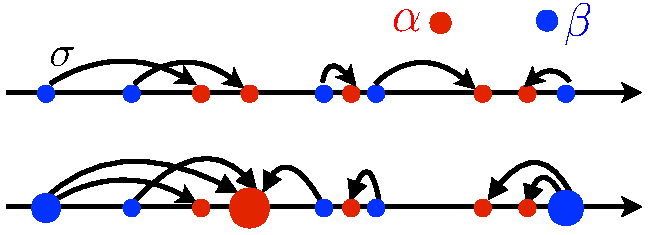
\includegraphics[width=.4\linewidth]{1d-discrete/1d-schematic}
%\caption{\label{fig-1d-discrete}
%1-D optimal couplings: each arrow $x_i \rightarrow y_j$ indicate a non-zero $\P_{i,j}$ in the optimal coupling.
%% 
%Top: empirical measures with same number of points (optimal matching).
%Bottom: generic case. 
%%
%This corresponds to monotone rearrangements, if $x_i \leq x_{i'}$ are such that $\P_{i,j} \neq 0, \P_{i',j'} \neq 0$, then necessarily $y_j \leq y_{j'}$.
%}
%\end{figure}


%%%%%%%%%%%%%%%%%%%%%%%%%%%%%%%%%%%%%%%%%%%%%%%%%%%%%%%%%%%%%%%%%%%%%%%%%%%
\subsection{Matching Algorithms}

There exists efficient algorithms to solve the optimal matching problems. The most well known are the hungarian and the auction algorithm, which runs in $O(n^3)$ operations. Their derivation and analysis is however very much simplified by introducing the Kantorovitch relaxation and its associated dual problem.
%
A typical application of these methods is the equalization of the color palette between images, which corresponds to a 3-D optimal transport. 

  
  
  